\section{A Rotating LED Display}
This section will deal with the, perhaps, most important part of the project.
Namely, the display.
The choice of electronics components for the display is presented along with the reasoning behind each choice.
Additionally, some compromises that were made are explained.

\subsection{Choosing the Components}
The components were chosen based on a series of requirements.
These are mentioned as they become relevant in the following paragraphs.

\paragraph{LED:}
Naturally, an LED display requires LEDs.
One requirement for the display is that it should be capable of displaying simple images at a reasonable resolution.
Reaching higher resolutions can be done either by increasing the display size and moving further away, or by increasing the "pixel" density.
In this case the latter was chosen since the version of Eagle, the software used to lay out the boards used in this project, does not allow for larger than 10$\times$10 cm boards.
Increasing "pixel" density in this case means to shrink down the LEDs and position them closer to one another.
This resulted in choosing an SMD LED.
Additionally the choice was made to use an RBG variant.
Finally, the choice fell on an Osram RGB LED.
20 of these mounted on a board will constitute the display.

When laying out the board however, it was found that the recommended footprint of this component is far bigger than the component itself.
See figure \ref{fig:recommendedfootprint}.
Using this footprint would severely limit the ability to position the LEDs as close as was intended.
The purpose of these larger pads is, while not explained in the datasheet, presumably to dissipate the heat generated by the component.
By driving the LEDs at lower currents and thereby generating less heat, it is assumed to be safe to reduce the size of the footprint.
While it may reduce the lifespan of the LEDs significantly if they run hotter than intended, it is unlikely to damage them within the time given for the project.
The footprint created for the component can be seen in figure 
\ref{fig:finalfootprint}.

\begin{figure}[H]
	\begin{subfigure}[t]{.49\linewidth}
		\centering
		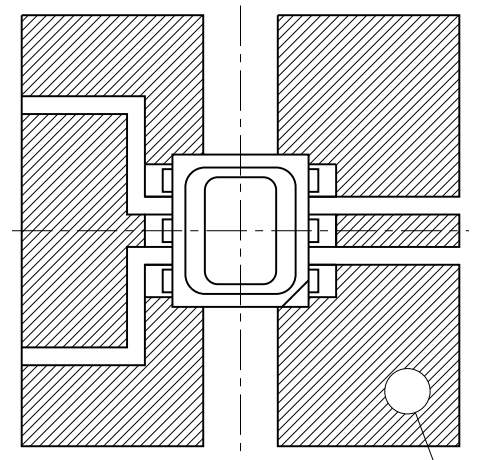
\includegraphics[width=.8\linewidth]{images/rgbfootprint}
		\caption{Recommended footprint.}
		\label{fig:recommendedfootprint}
	\end{subfigure}
	\begin{subfigure}[t]{.49\linewidth}
		\centering
		
\includegraphics[width=.8\linewidth]{images/stop}
		\caption{Reduced size footprint.}
		\label{fig:finalfootprint}
	\end{subfigure}
	\caption{Footprint of the Osram RGB LED.}
	\label{fig:footprint}
\end{figure}

\paragraph{LED Driver:}
Having 20 RGB LEDs that should all be individually controlled requires 60 control signals.
This is far more than what is available on the FPGA.
For this reason an LED driver is needed.
